\section{Battle Script, el lenguaje de dominio específico para ejecutar el proyecto}

El usuario final del proyecto necesita un medio para específicar las condiciones del enfrentamiento a simular, entiéndase cómo son las unidades, los soldados, el mapa, el movimiento de las unidades, etcétera. Para ello se implementó un lenguaje de dominio específico (DSL, por sus siglas en inglés \textit{Domain Specific Language}) con el nombre de Battle Script, que permite la creación de nuevas unidades, la creación de obstáculos, la creación de mapas, la inserción de unidades y obstáculos en el mapa, la creación de bandos, y la ejecucción de la simulación.

\subsection{Gramática}

Se diseñó la siguiente gramática para el lenguaje:

\begin{verbatim}
bs_file ->  classes statements EOF     
    |   EOF                       

classes -> class_def  classes         
    |  class_def                       

statements ->   statement  statements      
        |   statement                       

statement ->    func_def
        |   if_def
        |   while_def
        |   decl  ';' 
        |   assign  ';' 
        |   return_stat  ';' 
        |   'break'    ';'                        
        |   'continue'  ';'                       
        |   expressions ;


func_def ->     'function' return_type NAME '(' params ')' '->' block       
        |   'function' return_type NAME '(' ')' '->' block              

if_def ->   'if' expression '->' block elif_def                             
    |   'if' expression '->' block else_def                             
    |   'if' expression '->' block                                      

elif_def ->     'elif' expression '->' block elif_def                       
        |   'elif' expression '->' block else_def                       
        |   'elif' expression '->' block                                

else_def -> 'else' '->' block                                               

class_def ->    'class' NAME 'is' NAME '->' '{'  constructor functions '}'   
    |       'class' NAME 'is' NAME '->' '{'  constructor '}'                     


functions -> func_def  functions                     
       | func_def                                

constructor -> 'constructor' '(' params ')' '->' '{' attributes '}'              
         | 'constructor' '(' ')' '->' '{'  attributes '}'                 
         | 'constructor' '(' ')' '->' '{' '}'                   


attributes -> attr_def  attributes             
        | attr_def                         

attr_def ->  type 'this' '.' NAME '=' expression ';'          


while_def ->    'while' expression '->' block              

return_type ->  'void'                        
        |   type                          

type ->   'number'        
  |   'bool'          
  |   NAME            

assign -> NAME '=' expression                         

decl ->  type NAME '=' expression                              

return_stmt ->  'return' expression                                      
        |   'return'                                        

block ->     '{' statements '}'   

params ->   type NAME ',' params      
    |  type NAME                  


expressions ->  expression ','  expressions               
        |   expression                                

expression ->   disjunction 'if' disjunction 'else' expression            
        |   disjunction                                                

disjunction ->  conjunction 'or' disjunction                                
        | conjunction                                                   

conjunction ->  inversion 'and' conjunction                                 
        |   inversion                                                   

inversion ->    'not' inversion                                             
        |    comparision                                                


comparision ->  sum compare_par                                            
        |   sum

compare_par ->  'eq' sum                        
        |   'neq' sum                       
        |   'lte' sum                       
        |   'lt' sum                        
        |   'gte' sum                       
        |   'gt' sum                        


sum ->  sum '+' term                            
    |   sum '-' term                            
    |   term 

term -> term '*' factor                         
    |   term '/' factor                         
    |   term '%' factor                         
    |   factor

factor ->   '+' factor
    |   '-' factor
    |   pow

pow ->  primary '^' factor              
    |   primary

primary ->  primary '.' NAME            
    |   primary '(' args ')'        
    |   primary '(' ')'             
    |   atom

args -> expression ',' args
    | expression

atom -> NAME                            
    |   'True'                          
    |   'False'                         
    |   'None'                          
    |   NUMBER                          
    |   list

list -> '[' expressions ']'             
    |   '[' ']'                         
\end{verbatim}

\subsection{Compilador}

% TODO: ESCRIBIR MUELA BISCA DEL COMPILADOR
AQUI VA UNA MUELA BISCA DE CóMO ES EL COMPILADOR A GRANDES RASGOS

\subsection{Tokenizador}

Un Tokenizador, comúnmente llamado Lexer, es un ente encargado de dividir la cadena de texto de entrada del compilador en tokens del alfabeto del lenguaje Battle Script, identificando el tipo del token y envíandolo a la siguiente etapa del proceso de compilación.

Para la implementación del tokenizador fue necesario un sistema de expresiones regulares, una clase para representar un token, así como su tipo y la definición de los tokens del lenguaje, además de la clase propia del tokenizador. 

\subsubsection{Sistema de expresiones regulares}

Una expresión regulares es una definición recursiva de un lenguaje donde $a$ es la expresión regular para $L(a) = \{a\}$ y $\epsilon$ es la expresión regular para $L(\epsilon) = \{\epsilon\}$. Si $s$ y $r$ son expresiones regulares entonces:

\begin{itemize}
    \item $(s)|(r)$ es la expresión regular para la unión de lenguajes $L(s) \cup L(r)$
    \item $(s)(r)$ es la expresión regular para la concatenación de lenguajes $L(s)L(r)$
    \item $(s)*$ es la expresión regular para la clausura del lenguaje $L(s)* = \bigcup\limits_{k=0}^{\infty} L(s)^k$
\end{itemize}

Se implementó un sistema de expresiones regulares que admite los siguientes operadores:

\begin{itemize}
    \item $|$ que hace la unión de dos expresiones regulares.
    \item La concatenación de expresiones regulares de la siguiente forma, si $a$ y $b$ son expresiones regulares entonces $ab$ es la expresión de la concatenación.
    \item $*$ que hace la clausura del lenguaje que representa la expresión regular.
    \item $?$ que busca la coincidencia de la expresión regular una vez o ninguna.
    \item $+$ que busca la coincidencia de la expresión regular una o más veces.
    \item $.$ que busca la coincidencia de ninguno o cualquier caracter.
    \item $\setminus$  que permite la inclusión de los operadores anteriores en un expresión regular como un caracter.
\end{itemize}

La gramática para el lenguaje de las expresiones regulares que se implementó es la siguiente:

\begin{verbatim}
    regex = exp 

    exp      = term '|' exp    
            | term

    term     = factor term       
            | factor

    factor   = primary '*'      
            | primary '+'       
            | primary '?'       
            | primary

    primary  = '(' exp ')'
            | '\' CHAR              
            | CHAR
            | '.'
\end{verbatim}

Una expresión regular en el sistema se implementó utilizando la clase \verb|Regex| de Python. Una expresión regular se construye con la cadena de texto que representa el patrón de la expresión regular. Este patrón se compila y se devuelve un Autómata Finito No Determinista (NFA) que se utiliza para los procesos de saber si una cadena pertenece al lenguaje representado por la expresión, o encontrar todas las coincidencias de la expresión en una cadena de texto. 

\begin{verbatim}
class Regex:
        def __init__(self, pattern: str):
            self.pattern : str = pattern
            self.nfa : NFA = self.compile()
    
        def compile(self) -> NFA:
            lex: Lexer = Lexer(self.pattern)
            parser : Parser = Parser(lex)
            tokens : List[Token] = parser()
            handler: Handler = Handler()
            
            nfa_stack : List[NFA]= []
            
            for t in tokens:
                handler.handlers[t.name](t, nfa_stack)
            
            if len(nfa_stack) == 1:
                return nfa_stack.pop() 
            raise Exception("Bad regex!")
    
        def match(self, string: str) -> bool:
            return self.nfa.match(string)
    
        def find_all(self, string: str) -> List[Match]:
            return self.nfa.find_all(string)
\end{verbatim}

El proceso de compilación de una expresión regular es bastante sencillo, se tiene un tokenizador que recorre la cadena y cada vez que encuentra un operador o un caracter devuelve el token correspondiente, si encuentra el operador de escape ($\setminus$) devuelve un token de tipo \verb|CHAR| con el caracter siguiente. El proceso de Parsing consiste en recibir el conjunto de tokens provenientes del tokenizador y llamar al método \verb|exp| que este parsea el no terminal del mismo nombre de la gramática y va parseando el resto de no terminales según corresponda, o sea, se implementó un Parsing Recursivo Descendente.

Luego del proceso de parsing y verificar que la secuencia de tokens es correcta, se recorre la secuencia de tokens y haciendo uso de la clase \verb|Handler| se construye el autómata de la expresión regular. 

La clase \verb|Handler| es la encargada de dado un conjunto de tokens construir el autómata correspondiente, para ello implementa un método para cada operador de la gramática, estos métodos saben construir el autómata que resulta de aplicar la operación a uno, dos o más autómatas según el operador. La clase implementa el algoritmo Thompson's construction para la construcción del 

\begin{itemize}
        \item \textbf{Reconcimiento de un caracter:} el método de la clase \verb|Handler| encargado de construir dicho autómata construye el estado inicial \verb|s0| y el final \verb|s1| y añade la transición con el caracter en cuestión, como se muestra en la figura siguiente:
                \begin{figure}
                        \centering
                        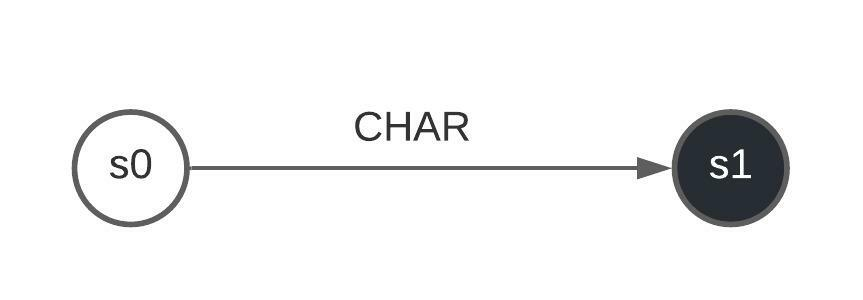
\includegraphics[width=6cm]{./chapters/img/char.jpeg}
                        \caption{Autómata finito no determinista para el reconocimiento de un caracter}
                \end{figure}
        \item \textbf{Operación de Unión:} el método encargado de construir el autómata solo debe los estados iniciales y finales, además añadir $\epsilon$-transiciones desde el estado incial hacia los autómatas y desde los autómatas hacia el estado final.
                \begin{figure}
                        \centering
                        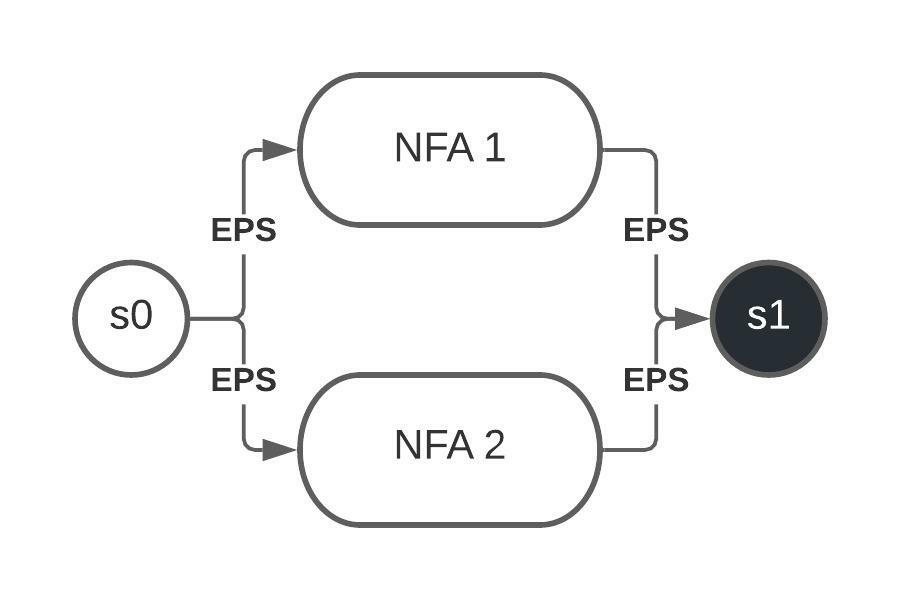
\includegraphics[width=6cm]{./chapters/img/alt.jpeg}
                        \caption{Autómata finito no determinista para el operador unión}
                \end{figure}
        \item \textbf{Operación de Concatenación:} el método encargado de construir el autómata solo debe  añadir una $\epsilon$-transición desde el estado final del primer autómata hacia el estado incial del segundo autómata.
                \begin{figure}
                        \centering
                        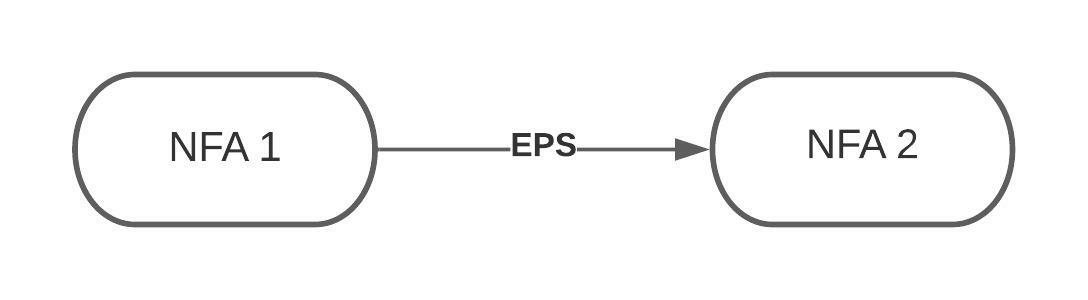
\includegraphics[width=6cm]{./chapters/img/concat.jpeg}
                        \caption{Autómata finito no determinista para el operador concatenación}
                \end{figure}
        \item \textbf{Operación} \verb|*|: el método encargado de construir el autómata solo debe los estados iniciales y finales, además añadir $\epsilon$-transiciones desde el estado incial hacia el autómata y desde el autómata hacia el estado final, así como una desde \verb|s0| hacia \verb|s1| para reconocer la no aparición del patrón, y una transición $\epsilon$ desde el estado final del autómata hacia el inicial para reconocer las repeticiones.
                \begin{figure}
                        \centering
                        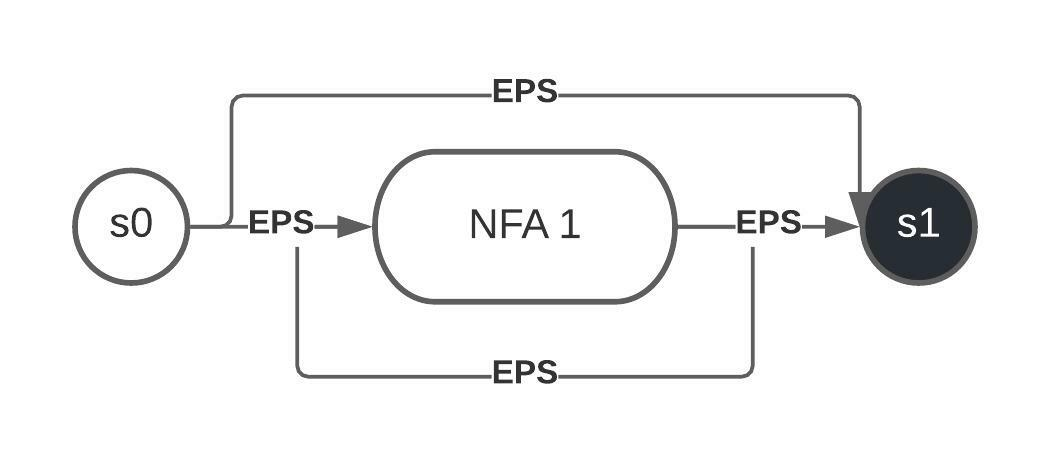
\includegraphics[width=6cm]{./chapters/img/star.jpeg}
                        \caption{Autómata finito no determinista para el operador *}
                \end{figure}
        \item \textbf{Operación} \verb|+|: el método encargado de construir el autómata solo debe los estados iniciales y finales, además añadir $\epsilon$-transiciones desde el estado incial hacia el autómata y desde el autómata hacia el estado final, y una transición $\epsilon$ desde el estado final del autómata hacia el inicial para reconocer las repeticiones.
                \begin{figure}
                        \centering
                        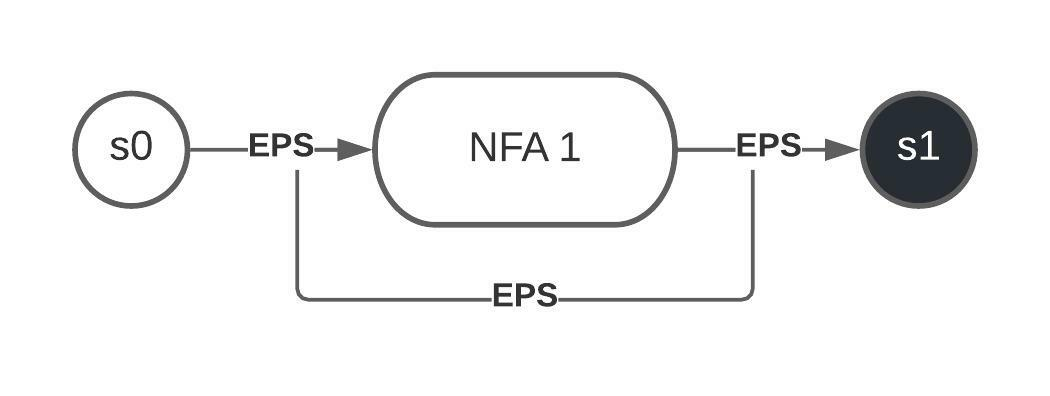
\includegraphics[width=6cm]{./chapters/img/plus.jpeg}
                        \caption{Autómata finito no determinista para el operador +}
                \end{figure}
        \item \textbf{Operación} \verb|.|: el método encargado de construir dicho autómata construye los estados inciales y finales ya añade un transición para cada caracter y añade un $\epsilon$-transición para reconocer la ocurrencia de ningún caracter. El autómata quedaría como el siguiente:
                \begin{figure}
                        \centering
                        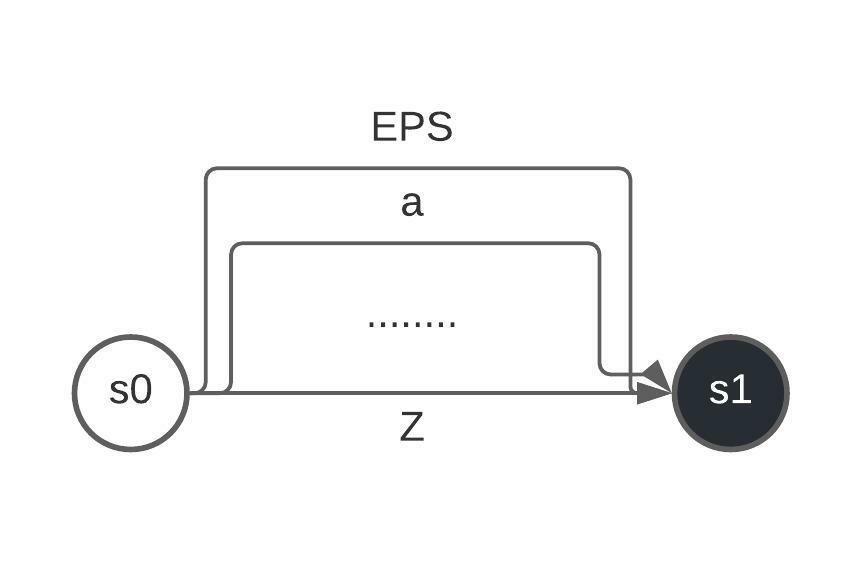
\includegraphics[width=6cm]{./chapters/img/dot.jpeg}
                        \caption{Autómata finito no determinista para el operador .}
                \end{figure}
        \item \textbf{Operación} \verb|?|: el método encargado de construir dicho autómata debe añadir una $\epsilon$-transición desde el estado incial del autómata hacia el estado final del autómata para reconocer la no aparición del patrón.
                \begin{figure}
                        \centering
                        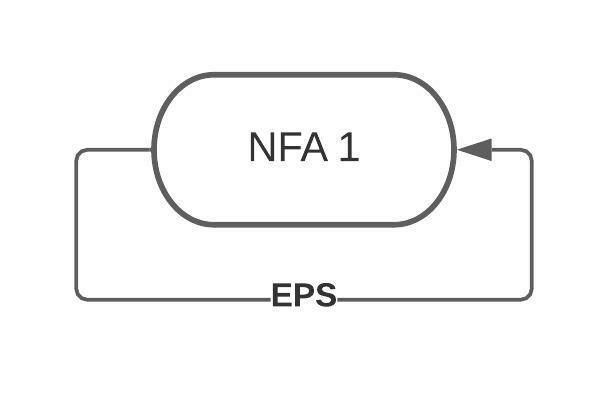
\includegraphics[width=6cm]{./chapters/img/qmark.jpeg}
                        \caption{Autómata finito no determinista para el operador ?}
                \end{figure}
\end{itemize}

Luego que se construye el autómata para una expresión regular  el proceso de compilación ha terminado. 

Entonces, ¿cómo saber si una cadena de texto pertence al alfabeto representado por una expresión regular? Para ello existen varios enfoques entre ellos están:

\begin{itemize}
        \item \textbf{Enfoque inocente o tonto:} utilizando backtracking y revisando los operadores y la cadena. Este enfoque es bien costo y no aprovecha las potencialidades de los autómatas anteriormente construidos.
        \item \textbf{Enfoque DFA:} se construye un Autómata Finito Determinista (DFA) a partir del no determinista anteriormente construido y se hace una pasada sobre él. Este enfoque es correcto, pero implica un procesamiento extra para construir el DFA.
        \item \textbf{Enfoque NFA:} este es el enfoque implementado en el proyecto en el método \verb|match| de una \verb|Regex|, que consiste en hacer una pasada sobre el autómata no determinista y revisar si coincide la cadena, pero el no determinismo trae un problema consigo, es que en un estado \verb|x| no se sabe con total seguridad que transición aplicar. Para ello, la propuesta es ejecutar las transiciones a la vez y ver si por alguna se llega al estado final. Esto hace que el tiempo de reconocimiento sea lineal respecto al tamaño de la cadena de entrada.
\end{itemize}

Entonces, ¿cómo encontrar todas las coincidencias de un patrón dentro de una cadena de texto?. Para ello se modificó el método anterior y cada vez que no se podía continuar  porque venía un caracter desconocido para la expresión regular se volvía al estado inicial. Además en cada posición se revisa si se ha llegado al estado final, se devuelve la coincidencia y se vuelve al estado inicial. Este procedimiento se implementó en método \verb|find_all| de las \verb|Regex|. Este procedimiento es lineal con respecto al tamaño de la cadena.

Luego de implementado el sistema de expresiones regulares se implementó la clase \verb|Token| y el enum \verb|TokenType|.

\subsubsection{Token y TokenType}

Un token en el proyecto se representa con la clase \verb|Token| que tiene la siguiente implementación. La propiedad \verb|regex| almacena la expresión regular que coincide con el token, la propiedad \verb|name| representa el nombre del tipo de token, la propiedad \verb|lexeme| almacena la cadena de texto que se extrajo de la cadena de entrada como token, es decir, si se tiene un token \verb|t| entonces \verb|t.regex.match(t.lexeme)| es verdadero. Además, un token almacena donde comienza y termina \verb|lexeme| en la cadena de entrada.

\begin{verbatim}
class Token:
        @propertyclass Token:
        @property
        def regex(self) -> Regex:
            return self.type.value[0]
    
        @property
        def name(self) -> str:
            return self.type.value[1]
            
        def __init__(self, token_type: TokenType, lexeme: str, start: int, end: int):
            self.type: TokenType = token_type
            self.lexeme: str = lexeme
            self.start: int = start
            self.end: int = end
        
    
        @property
        def name(self) -> str:
            return self.type.value[1]
            
        def __init__(self, token_type: TokenType, lexeme: str, start: int, end: int):
            self.type: TokenType = token_type
            self.lexeme: str = lexeme
            self.start: int = start
            self.end: int = end
        
\end{verbatim}

El tipo de los tokens se definió utilizando el enum \verb|TokenType| que representa la expresión regular que lo representa y el nombre del token, por ejemplo: para el token que representa la palabra reservada \verb|eq| el \verb|TokenType| correspondiente es \verb|Eq = (Regex("eq"), "eq")|

\subsubsection{Algoritmo del tokenizador}

El algoritmo del tokenizador sigue la siguiente idea general, se le asocia a cada token de la gramática un nivel de precedencia que representa cuán relevante es un token sobre otro. Por ejemplo si se tienen los siguientes: \verb|Token((Regex("eq"), "eq"), "eq", 1, 2)| y \texttt{Token((Regex("(a|b|....|Z)+"), "NAME"), 'eq', 1, 2)} donde el primer token tiene precedencia 1 y el segundo tiene 2, entonces el token más relevante es el primero. Entonces, se tiene una lista \verb|tokens| y se recorre la lista de tokens de la gramática y a cada uno se le piden todas coincidencias en la cadena de entrada. Luego se recorren las posiciones \verb|i| de la cadena de entrada, y se añade a \verb|tokens| aquel token que comience en \verb|i| y tenga menor precedencia.

\begin{verbatim}
class Tokenizer:
    def __call__(self, bs_content_file: str) -> Iterable[Token]:
        tokens: List[Token] = []

        matches = {}
        for token_def in TOKENS:
            matches[token_def] = token_def.type.value[0].find_all(bs_content_file)
        
        i = 0
        while i < len(bs_content_file):
            token_in_i: List[Tuple[TokenDefinition, Match]] = []

            # Get all matches
            for k, v in matches.items():
                for t in v:
                    if t.start == i:
                        token_in_i.append((k, t))
                    
            # Get match with highest precedence
            if len(token_in_i):
                token_in_i = sorted(token_in_i, key=lambda tup: tup[0].precendece)
                token = Token(token_in_i[0][0], \
                                token_in_i[0][1].value,\
                                token_in_i[0][1].start,\
                                token_in_i[0][1].end)
                tokens.append(token)    
                i = token.end

            i += 1
        return deque(tokens)
\end{verbatim}

Este algoritmo tiene complejidad temporal $O(n*m)$ donde $m$ es la cantidad de tokens, y $n$ el tamaño de la cadena de entrada.

\subsection{An\'alisis Sem\'antico}
\subsubsection{Definiendo tipos}
Para implementar nuevos tipos en el lenguaje se sigui\'o la idea de Python: se implement\'o una clase \verb|Type| en la que cada clase del lenguaje ser\'a una instancia de esta.
 
  \verb|Type| consta de los siguientes atributos y m\'etodos 
  \begin{itemize}
  \item Atributos
  \begin{itemize}
  \item \verb|name|: Nombre de la clase o nuevo tipo
  
  \item \verb|attributes|: Atributos de la clase.
  
  \item  \verb|methods|: M\'etodos de la clase
  \end{itemize}
  
  \item M\'etodos
  \begin{itemize}
  \item \verb|get_attribute|:  Devuelve el atributo de la clase que se pide si este existe.
  
  \item \verb|get_method|: Devuelve el m\'etodo de la clase que se pide si este existe.
  
  \item \verb|define_attribute|: Define el atriuto de la clase.
  
  \item \verb|define_method|: Define el m\'etodo de la clase.
  
  \item \verb|is_attribute|: Revisa si el atributo existe.
  
  \item \verb|is_method|: Revisa si el m\'etodo existe.
  \end{itemize}
  \end{itemize}
\subsubsection{Context}
Para definir en contexto en el que se escribe un programa con el lenguaje, se implement\'o la clase \verb|Context|, esta cuenta con los siguientes atributos y m\'etodos 
\begin{itemize}
\item Atributos
\begin{itemize}
\item \verb|father|: Contexto padre de este contexto

\item \verb|children|: Contextos hijos de este contexto

\item \verb|_var_context|: Variables del contexto. 

\item \verb|_func_context|: Funciones del contexto

\item \verb|_type_context|: Tipos definidos en el contexto
\end{itemize}

\item M\'etodos
\begin{itemize}
\item \verb|check_var|: Revisa si la variable est\'a definida en el contexto

	\item \verb|check_var_type|: Revisa que la variable est\'e definida en el contexto y el tipo corresponda con el tipo de la variable
	
	\item \verb|check_func|: Revisa que la funci\'on est\'e definida
	
	\item \verb|check_func_args|: Revisa si la funci\'on est\'a definida y los tipos de los argumentos coinciden con los tipos de la funci\'on
	
	\item \verb|get_type|: Devuelve el tipo de una variable en el contexto
	
	\item \verb|define_var|: Si la variable no existe en el contexto, la crea. En caso contrario le asigna el valor siempre que este corresponda con el tipo de la variable
	
	\item \verb|define_func|: Define la funci\'on si no existe en el contexto
	
	\item \verb|create_child_context|: Crea un contexto hijo
	
	\item \verb|create_type|: Crea un nuevo tipo en el contexto
	
	\item \verb|get_return_type|: Dvuelve el tipo de retorno de una funci\'on si esta est\'a definida en el contexto
	
	\item \verb|get_type_object|: Devuelve la clase a la que pertenece objeto dado 
\end{itemize}

\end{itemize}

\subsubsection{Visitor}
Para verificar la correcci\'on de la sem\'antica se implement\'o el patr\'on \verb|Visitor| que visitar\'a el \'arbol de sintaxis abstracta en tres pasadas distintas
\begin{itemize}
\item \verb|Type_Collector|: Es la primera pasada con el patr\'on \verb|Visitor| en este se recogen todos los tipos que se van a definir, para crearlos en el contexto

\item \verb|Type_Builder|: Es la segunda pasada con el patr\'on, se toman todos los tipos que se definieron anteriormente y se definen sus m\'etodos y atributos.

\item \verb|Type_Checker|: Es la tercera pasada con el patr\'on, en esta se revisan que los tipos de cada expresi\'on no entren en contradicci\'on
\end{itemize}